\appendix

%%%%%%%%%% DON'T DELETE THIS, REVERTS NUMBERING BACK %%%%%%%%%%%%%
\makeatletter
\renewcommand{\@makechapterhead}[1]{\vspace *{-10\p@ }{\parindent \z@ 
\raggedright \normalfont \ifnum \c@secnumdepth >\m@ne \Huge \bfseries 
\@chapapp \space \thechapter \vskip 10\p@ \fi #1\par \nobreak \vskip 30\p@ }}
\makeatother
%%%%%%%%%% DON'T DELETE THIS, REVERTS NUMBERING BACK %%%%%%%%%%%%%

% examples of appendix figures:
% \chapter{}
% \vspace*{-0.3in}
% \begin{figure}[hb!]
% \begin{center}
% \makebox[\textwidth][c]{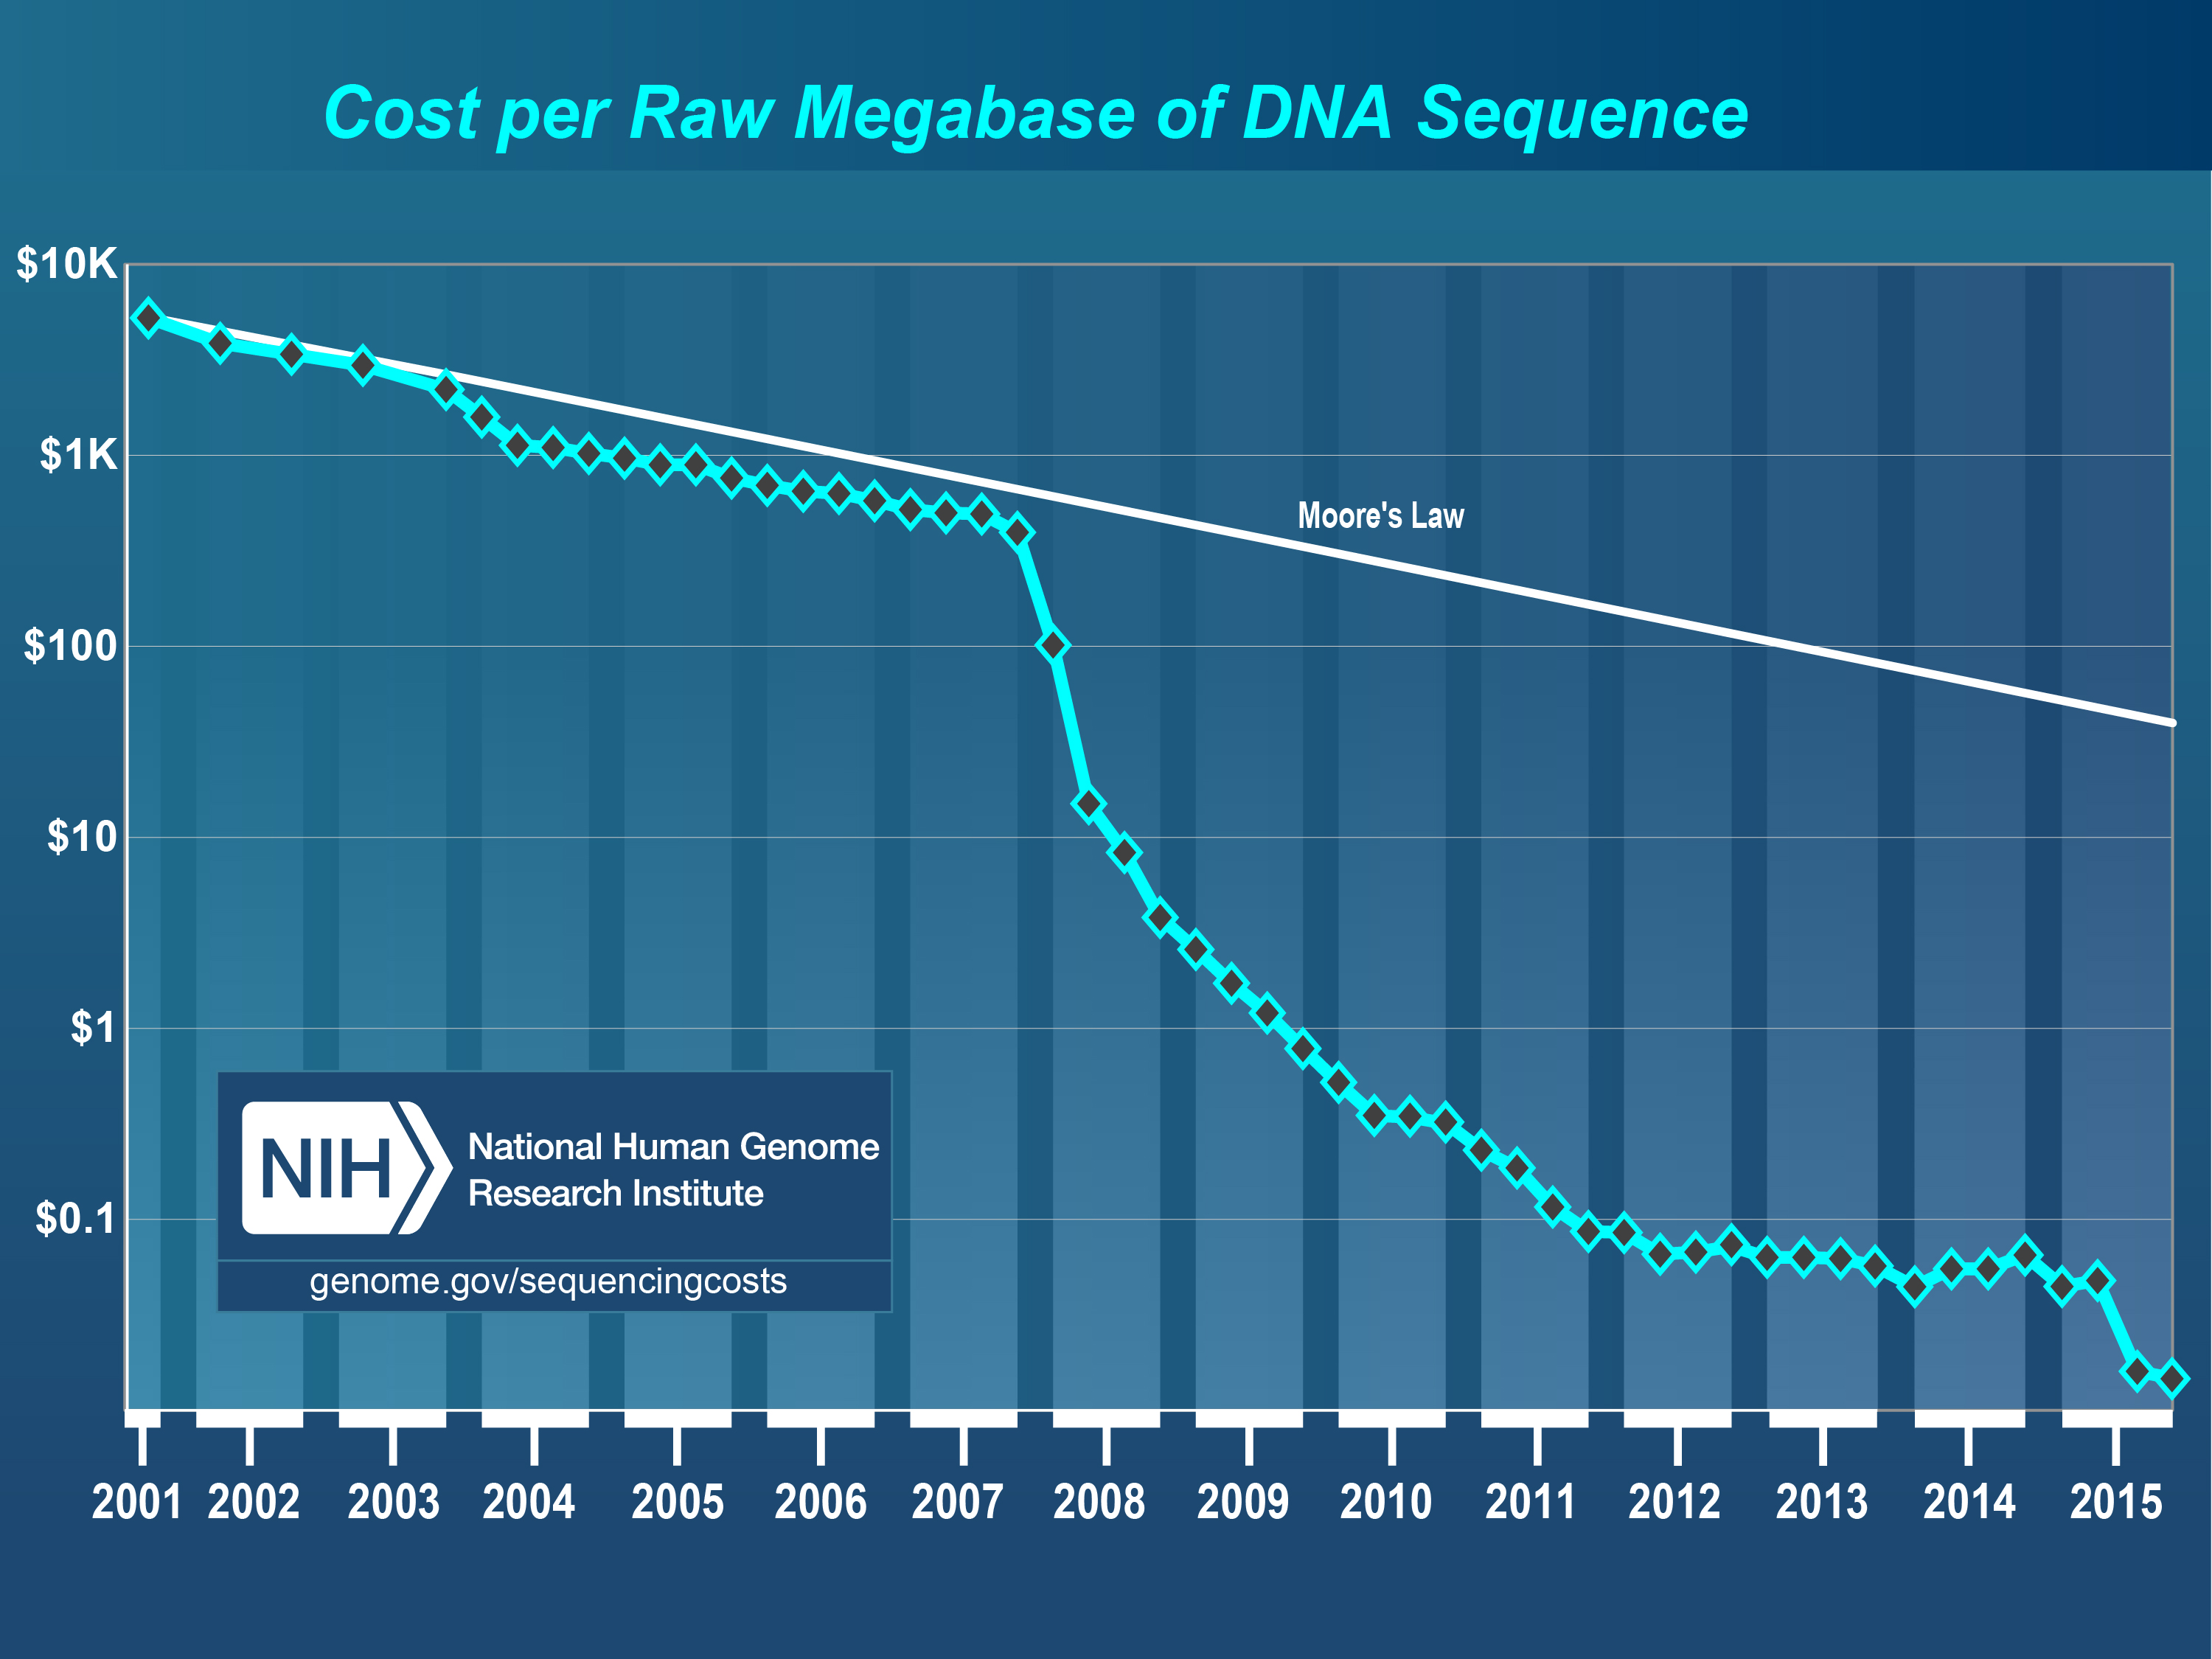
\includegraphics[width=1.0\textwidth]{costperMb2015_4.jpg}}
% \end{center}
% \caption[Cost per raw megabase of DNA sequence from 2001 to 2015]{Cost per raw megabase of DNA sequence from 2001 to 2015. Straight line - Moore's Law, blue curve - cost in US dollars, Y-axis scale is logarithmic. Graph reproduced from \citep{wetterstrand2016}}
% \end{figure}
% \begin{figure}[hb!]
% \begin{center}
% \makebox[\textwidth][c]{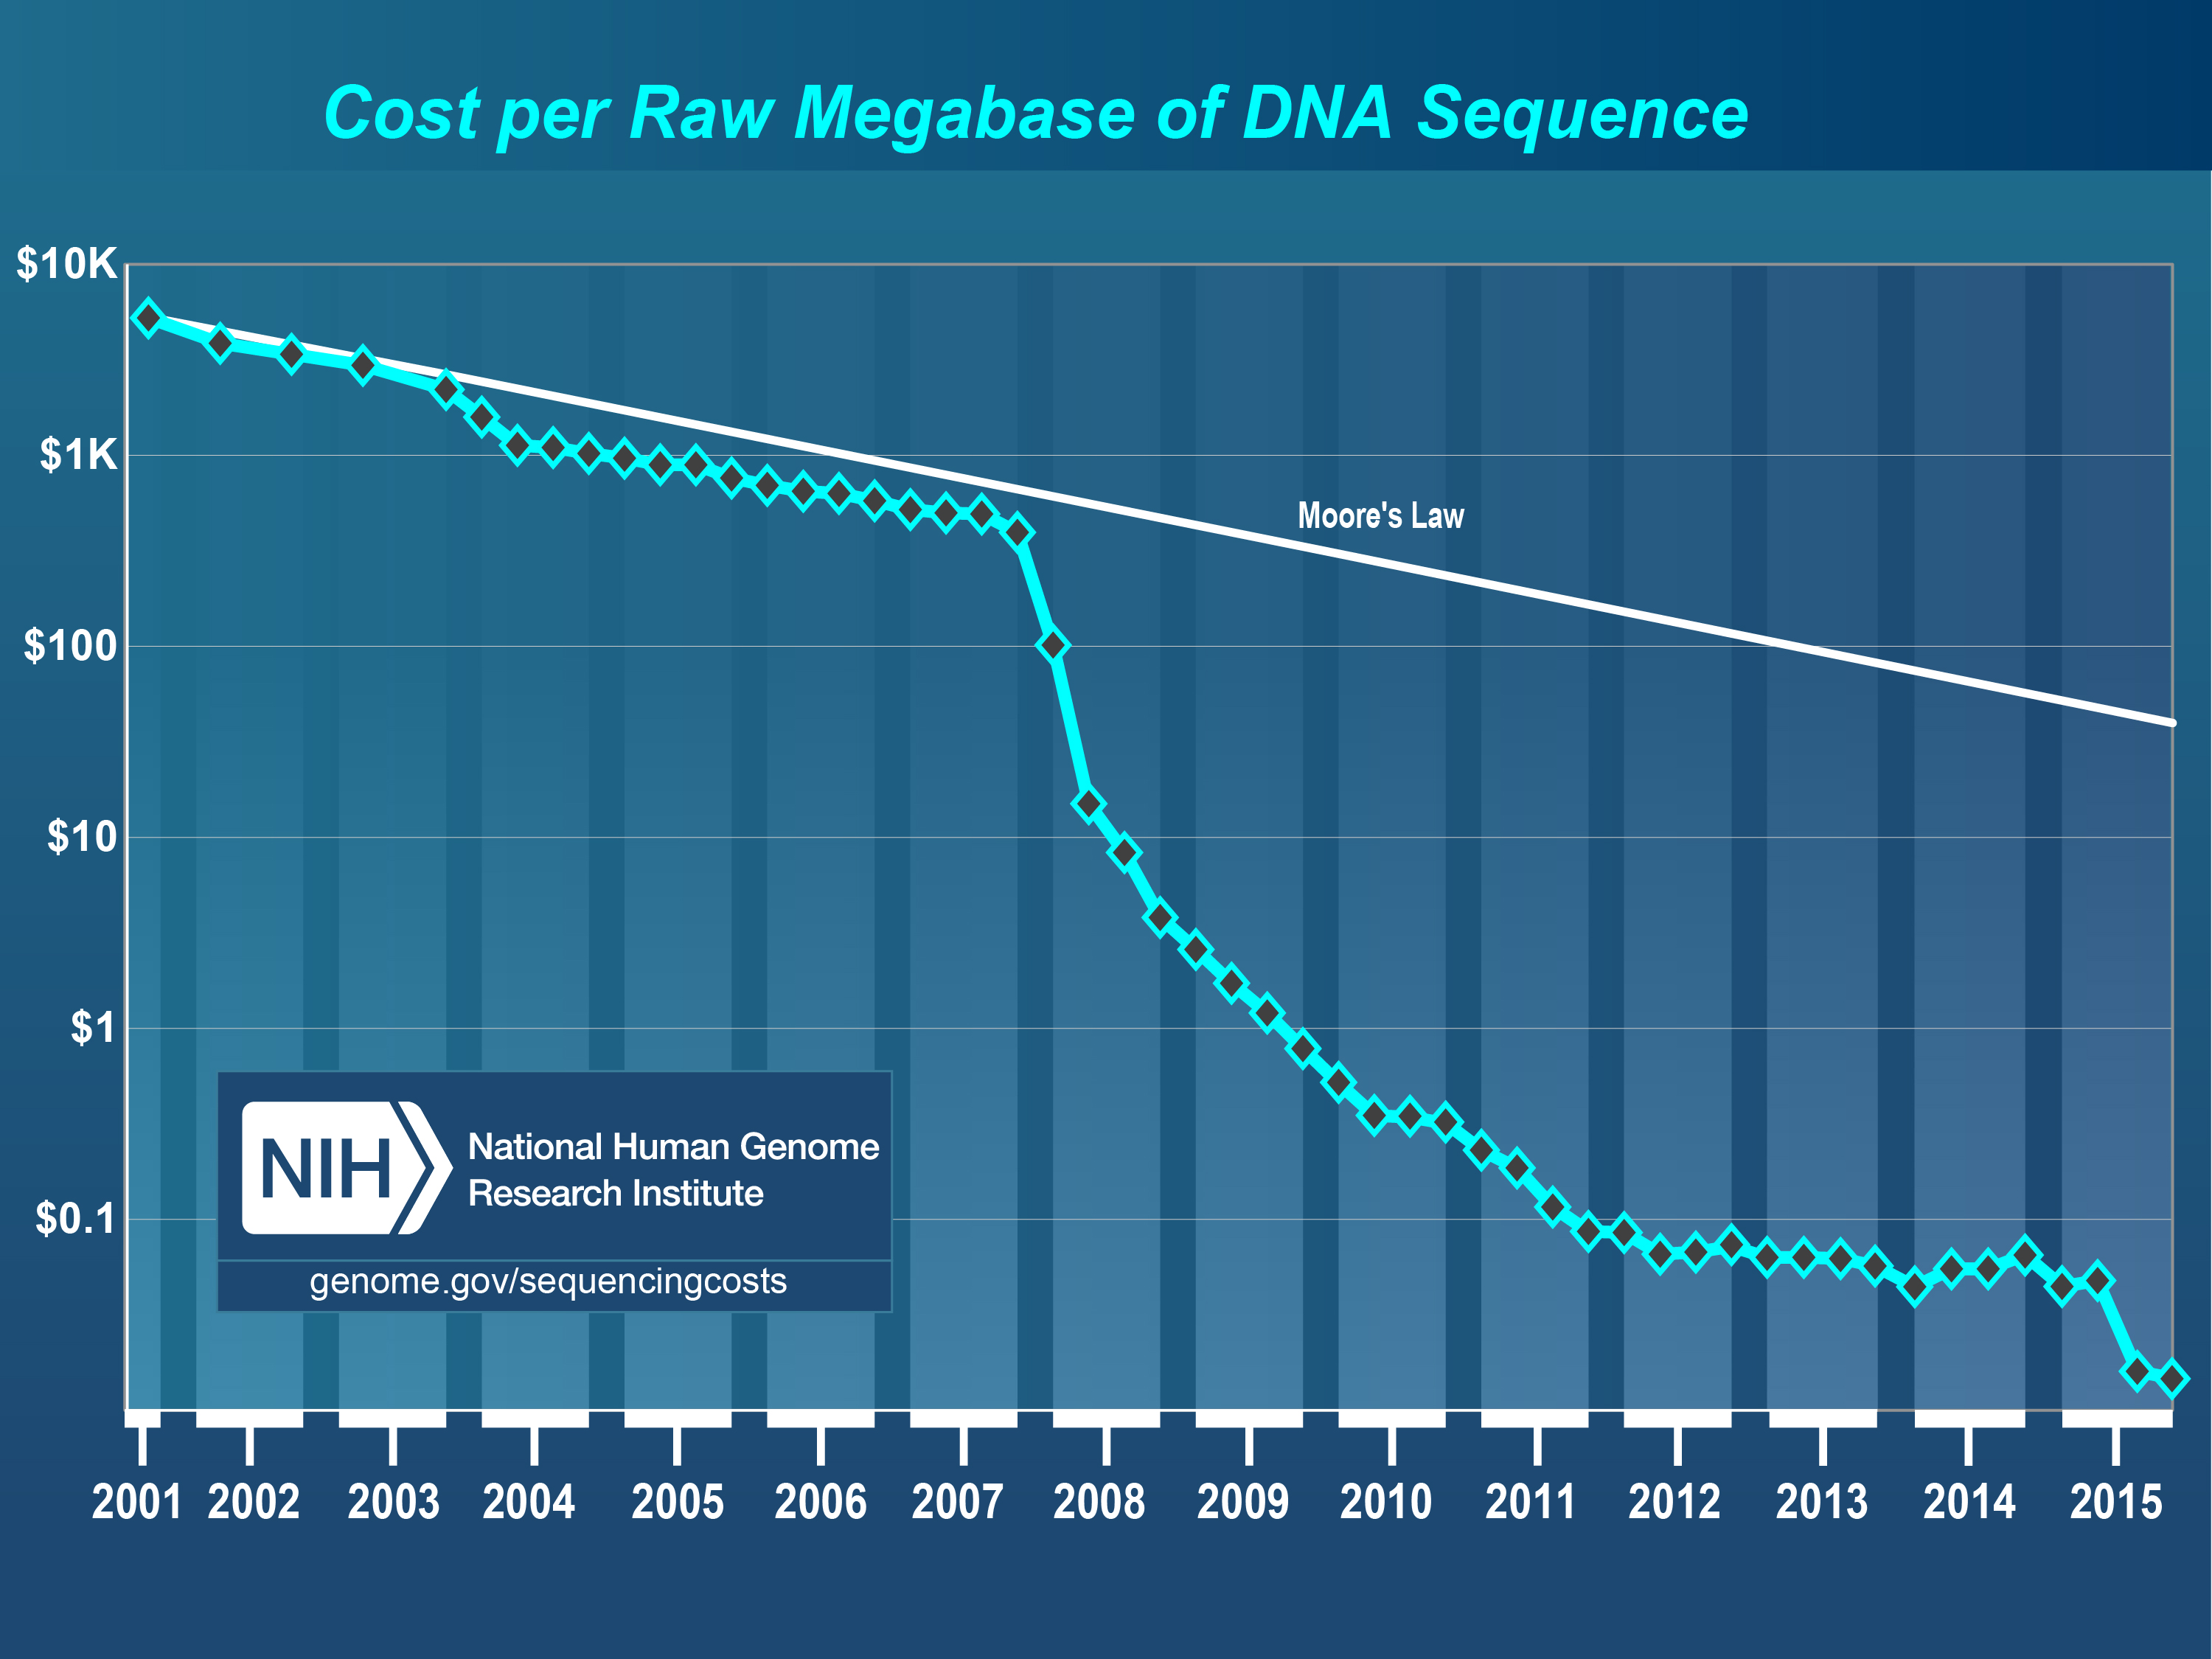
\includegraphics[width=1.0\textwidth]{costperMb2015_4.jpg}}
% \end{center}
% \caption[Cost per raw megabase of DNA sequence from 2001 to 2015]{Cost per raw megabase of DNA sequence from 2001 to 2015. Straight line - Moore's Law, blue curve - cost in US dollars, Y-axis scale is logarithmic. Graph reproduced from \citep{wetterstrand2016}}
% \end{figure}

% \chapter{}
% \vspace*{-0.3in}
% \begin{figure}[hb!]
% \begin{center}
% \makebox[\textwidth][c]{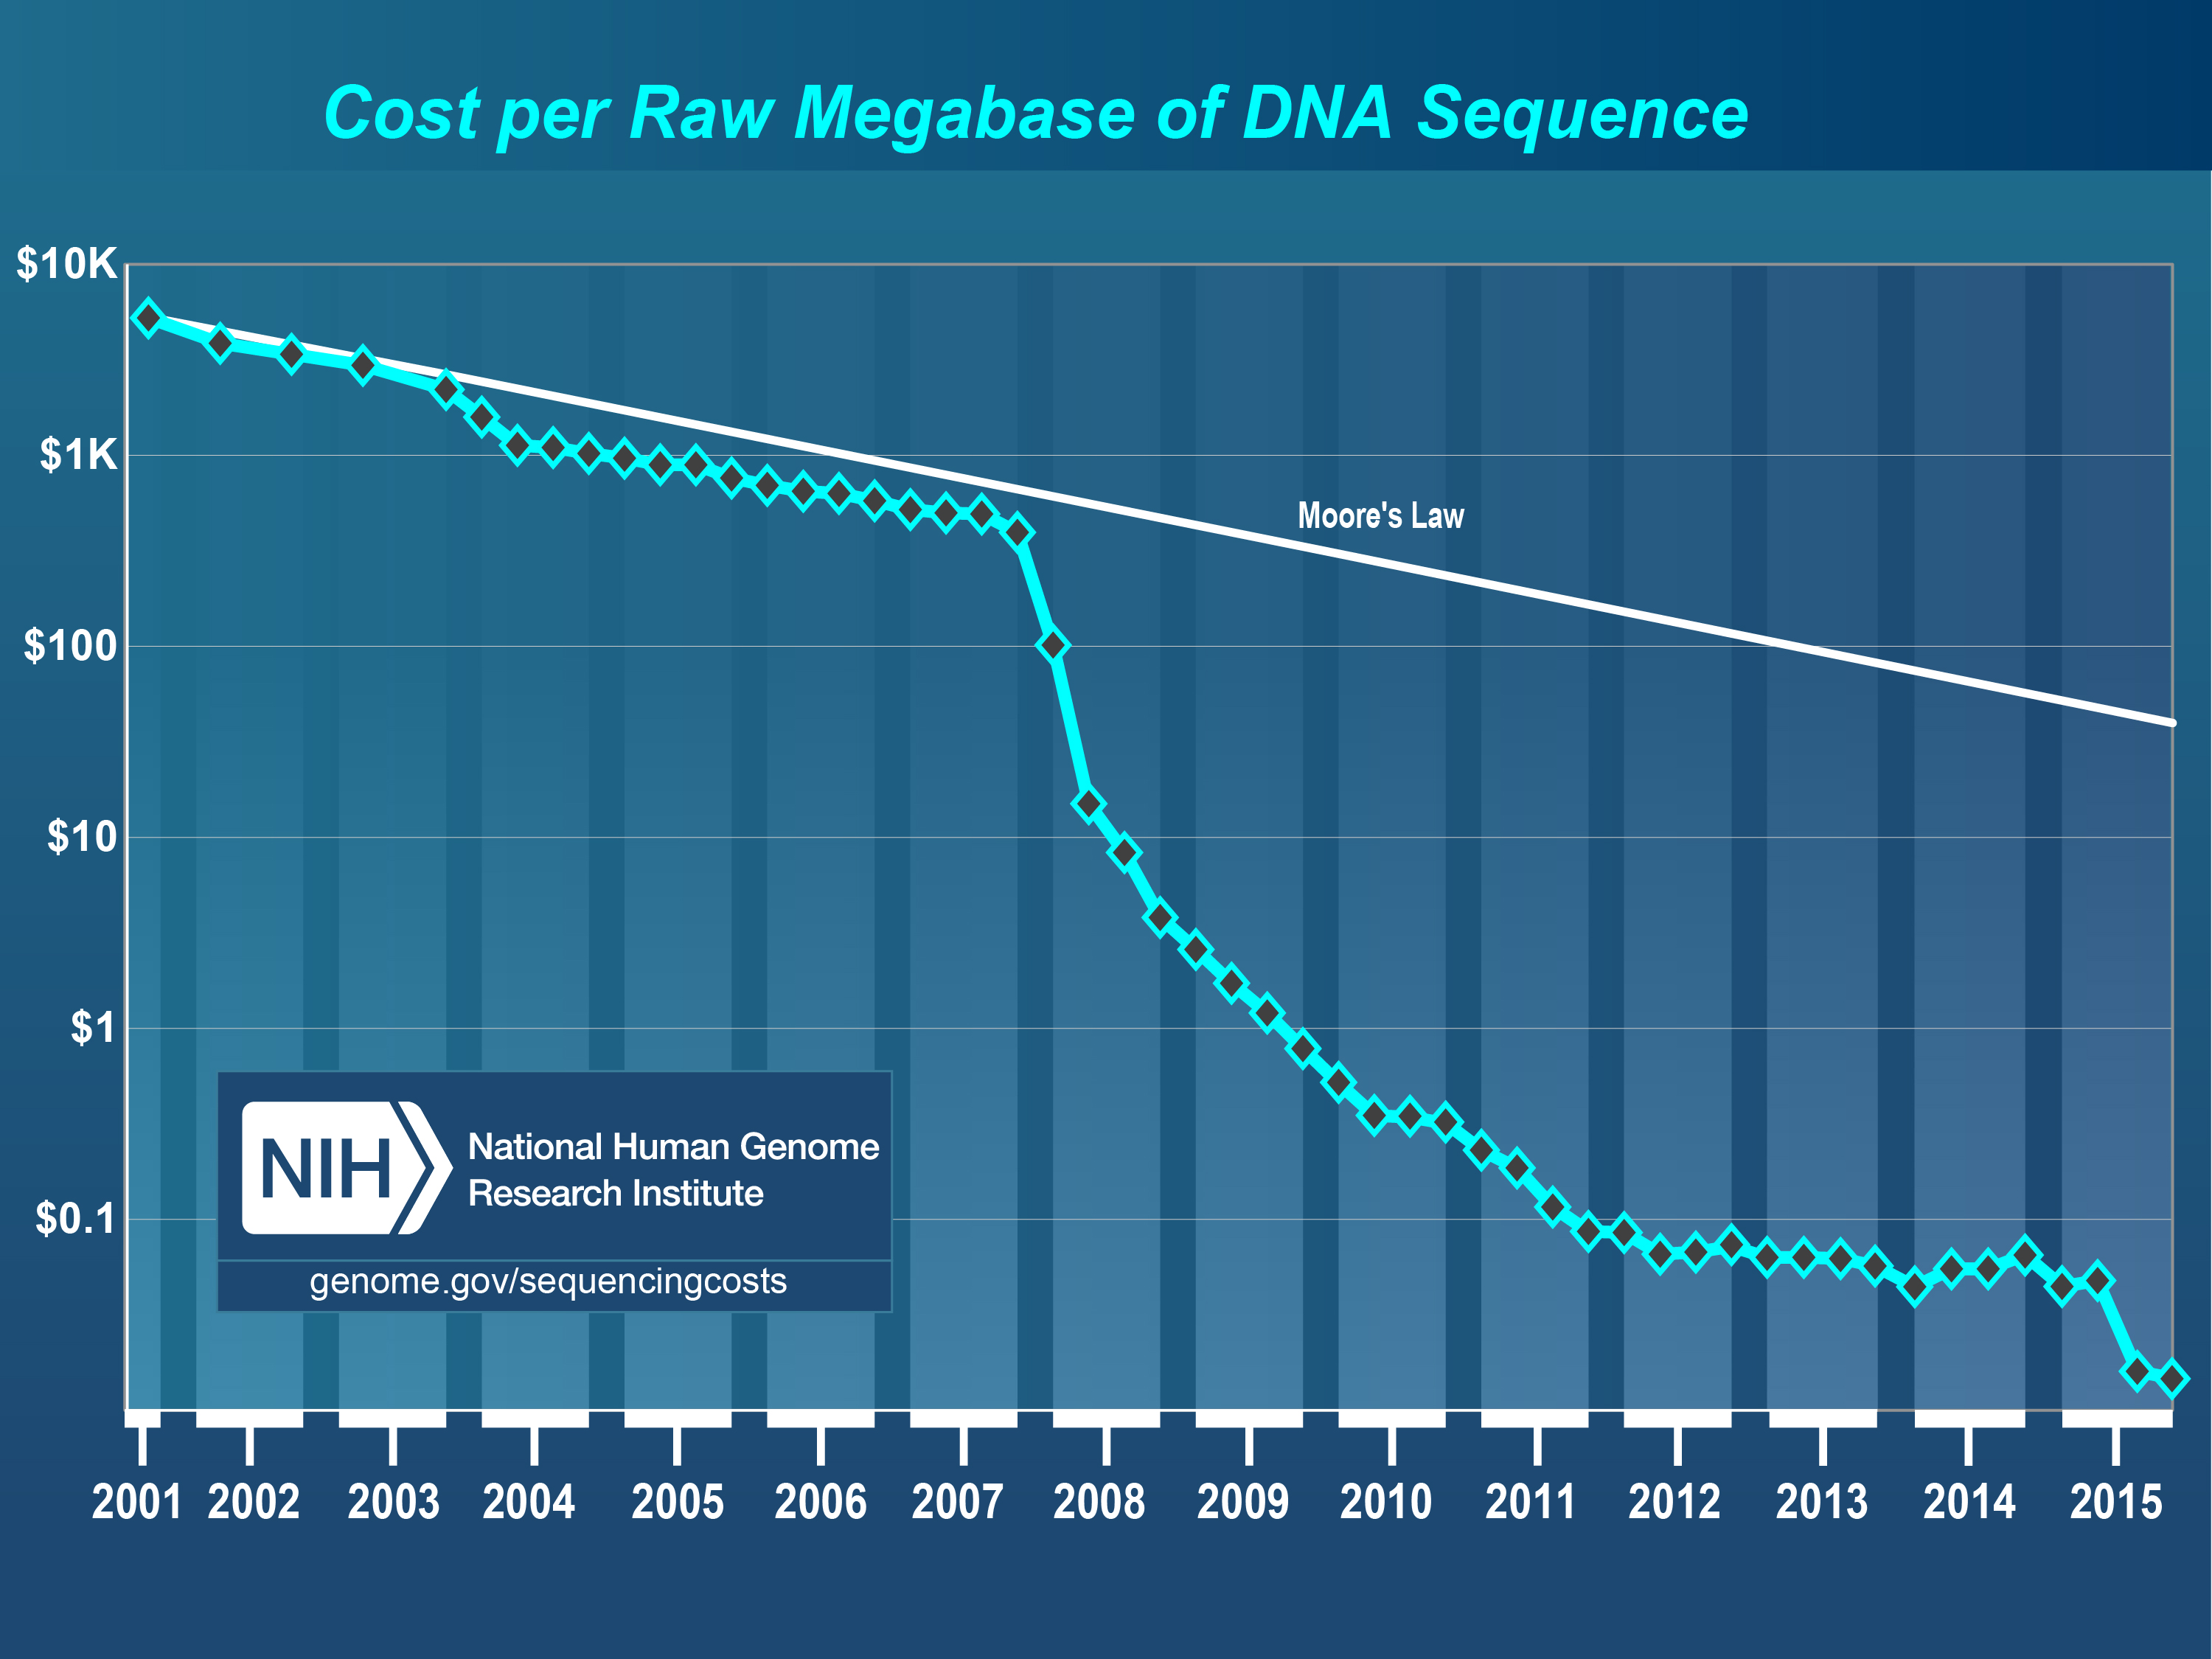
\includegraphics[width=1.0\textwidth]{costperMb2015_4.jpg}}
% \end{center}
% \caption[Cost per raw megabase of DNA sequence from 2001 to 2015]{Cost per raw megabase of DNA sequence from 2001 to 2015. Straight line - Moore's Law, blue curve - cost in US dollars, Y-axis scale is logarithmic. Graph reproduced from \citep{wetterstrand2016}}
% \end{figure}

% \chapter{}
% \begin{figure}[hb!]
% \begin{center}
% 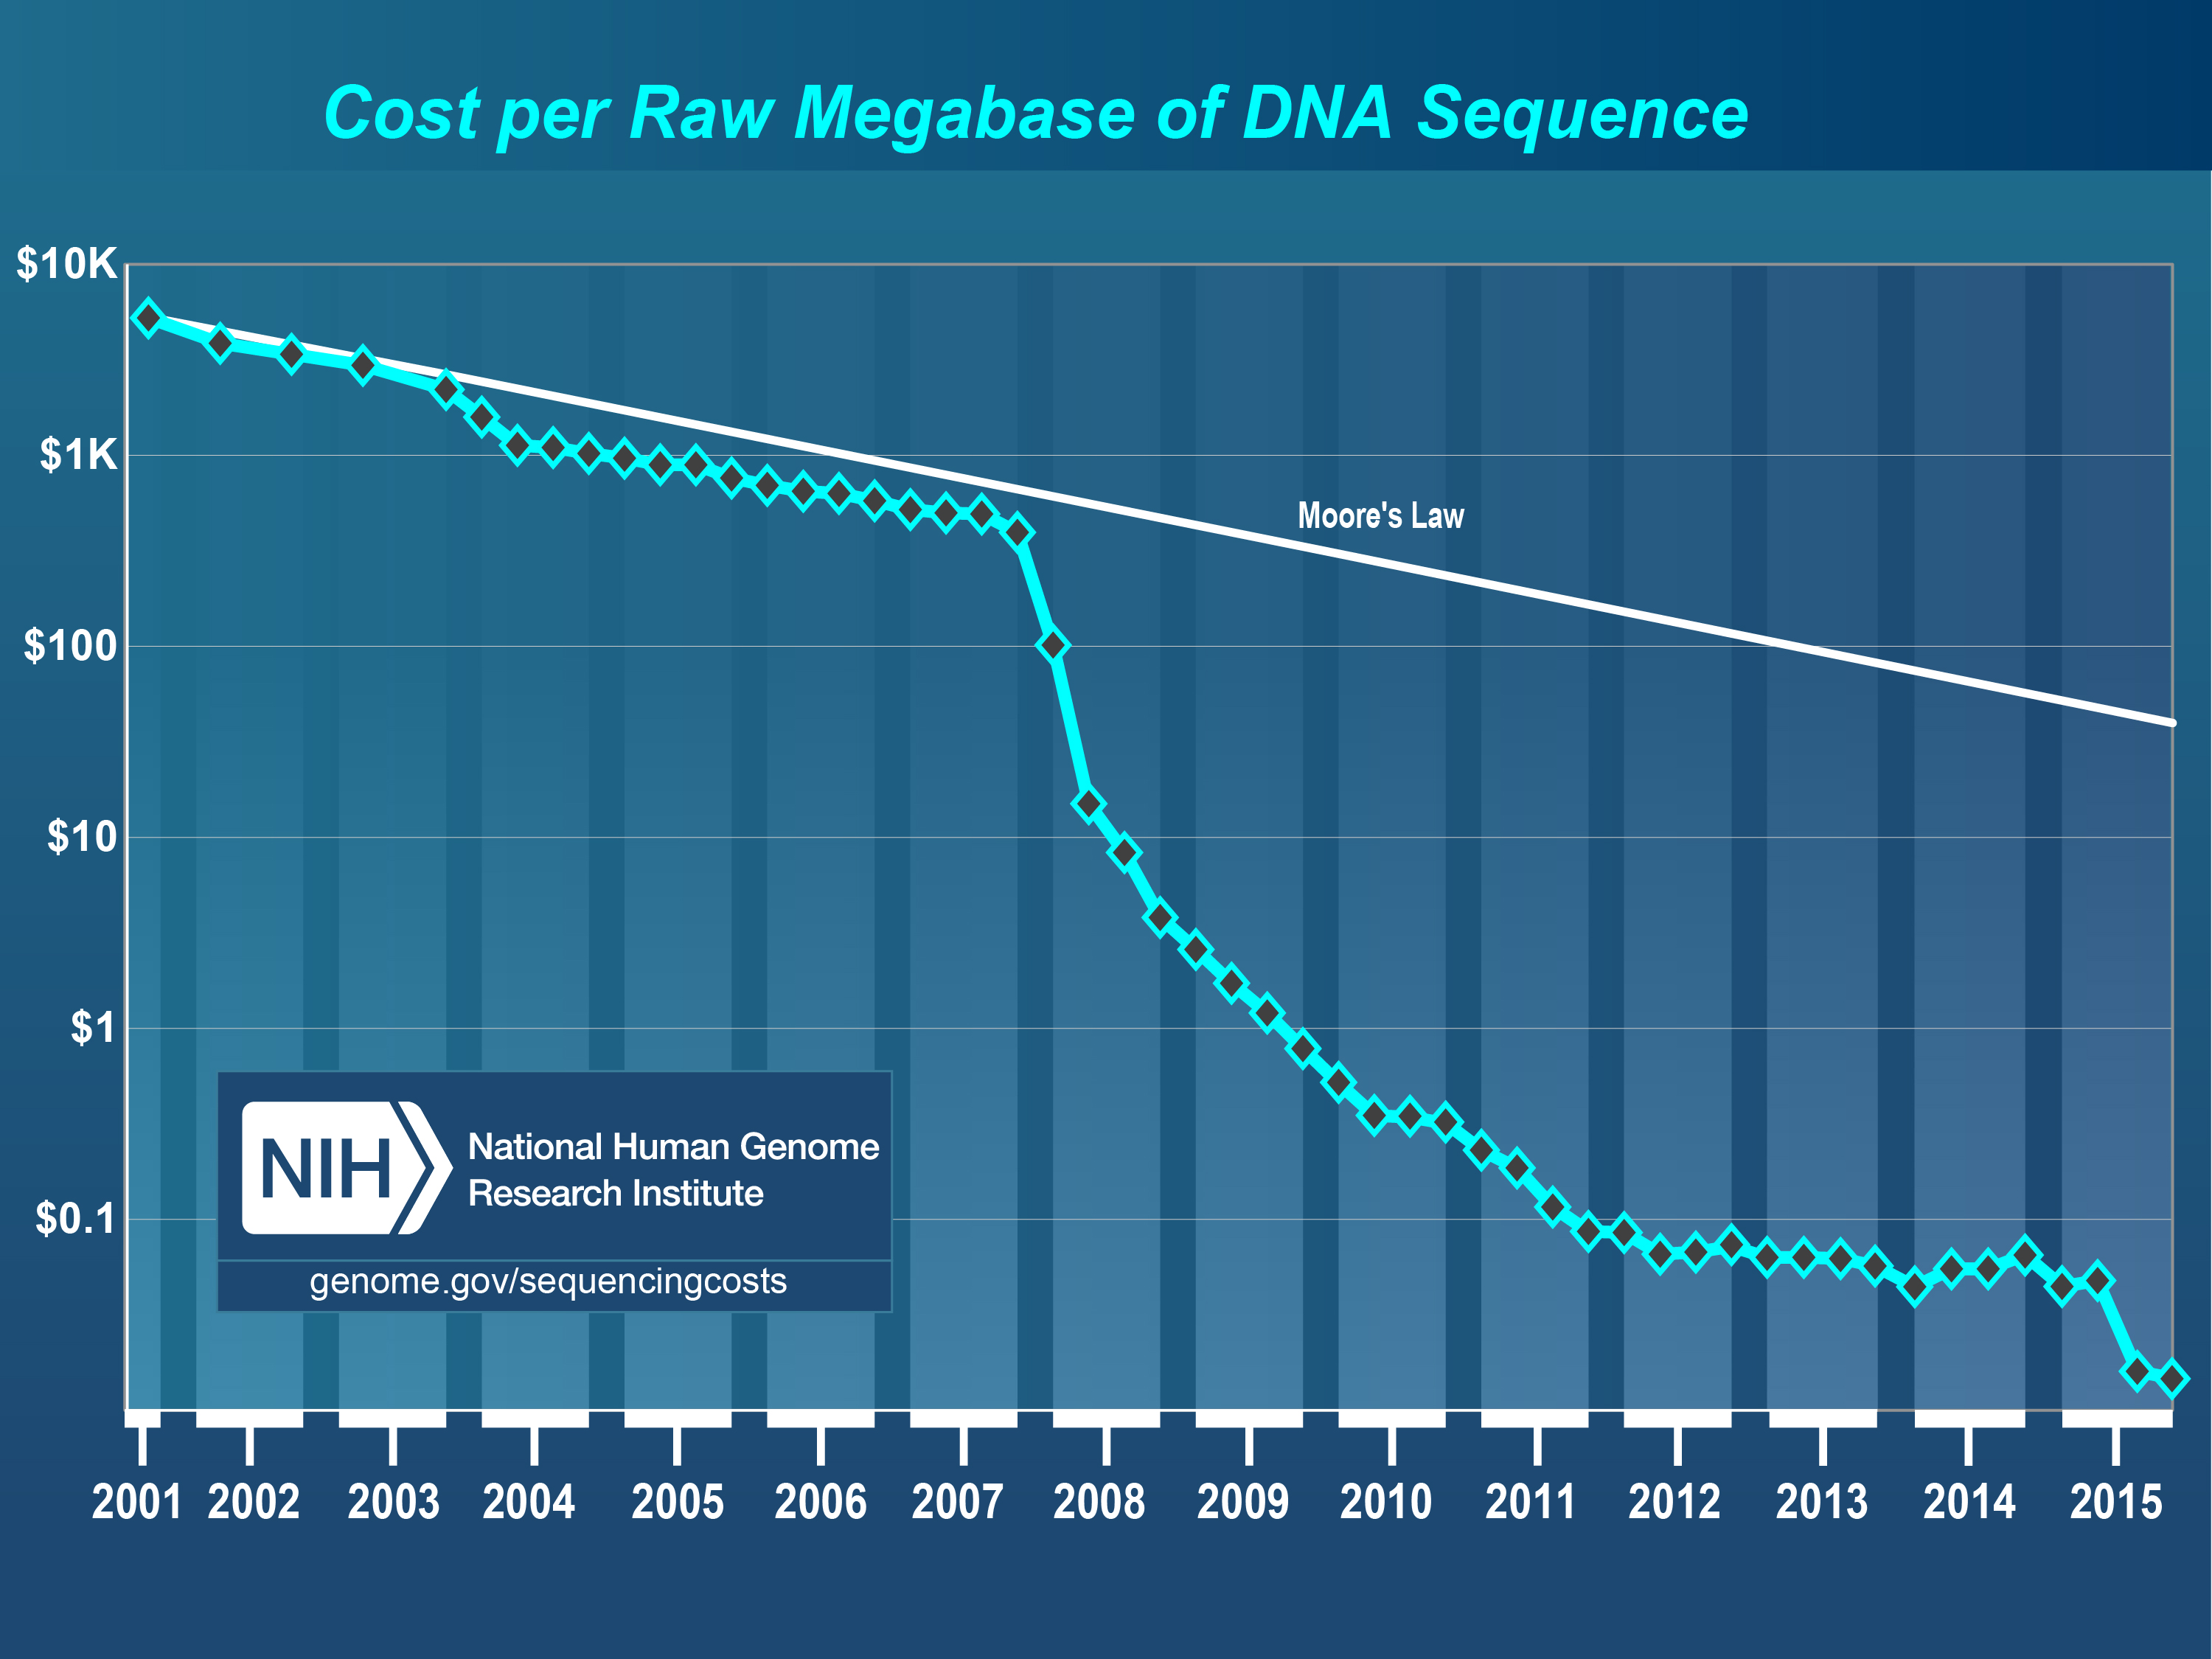
\includegraphics[scale=0.5]{costperMb2015_4.jpg}
% \end{center}
% \caption[Cost per raw megabase of DNA sequence from 2001 to 2015]{Cost per raw megabase of DNA sequence from 2001 to 2015. Straight line - Moore's Law, blue curve - cost in US dollars, Y-axis scale is logarithmic. Graph reproduced from \citep{wetterstrand2016}}
% \end{figure}

% \chapter{}
% \begin{figure}[hb!]
% \begin{center}
% 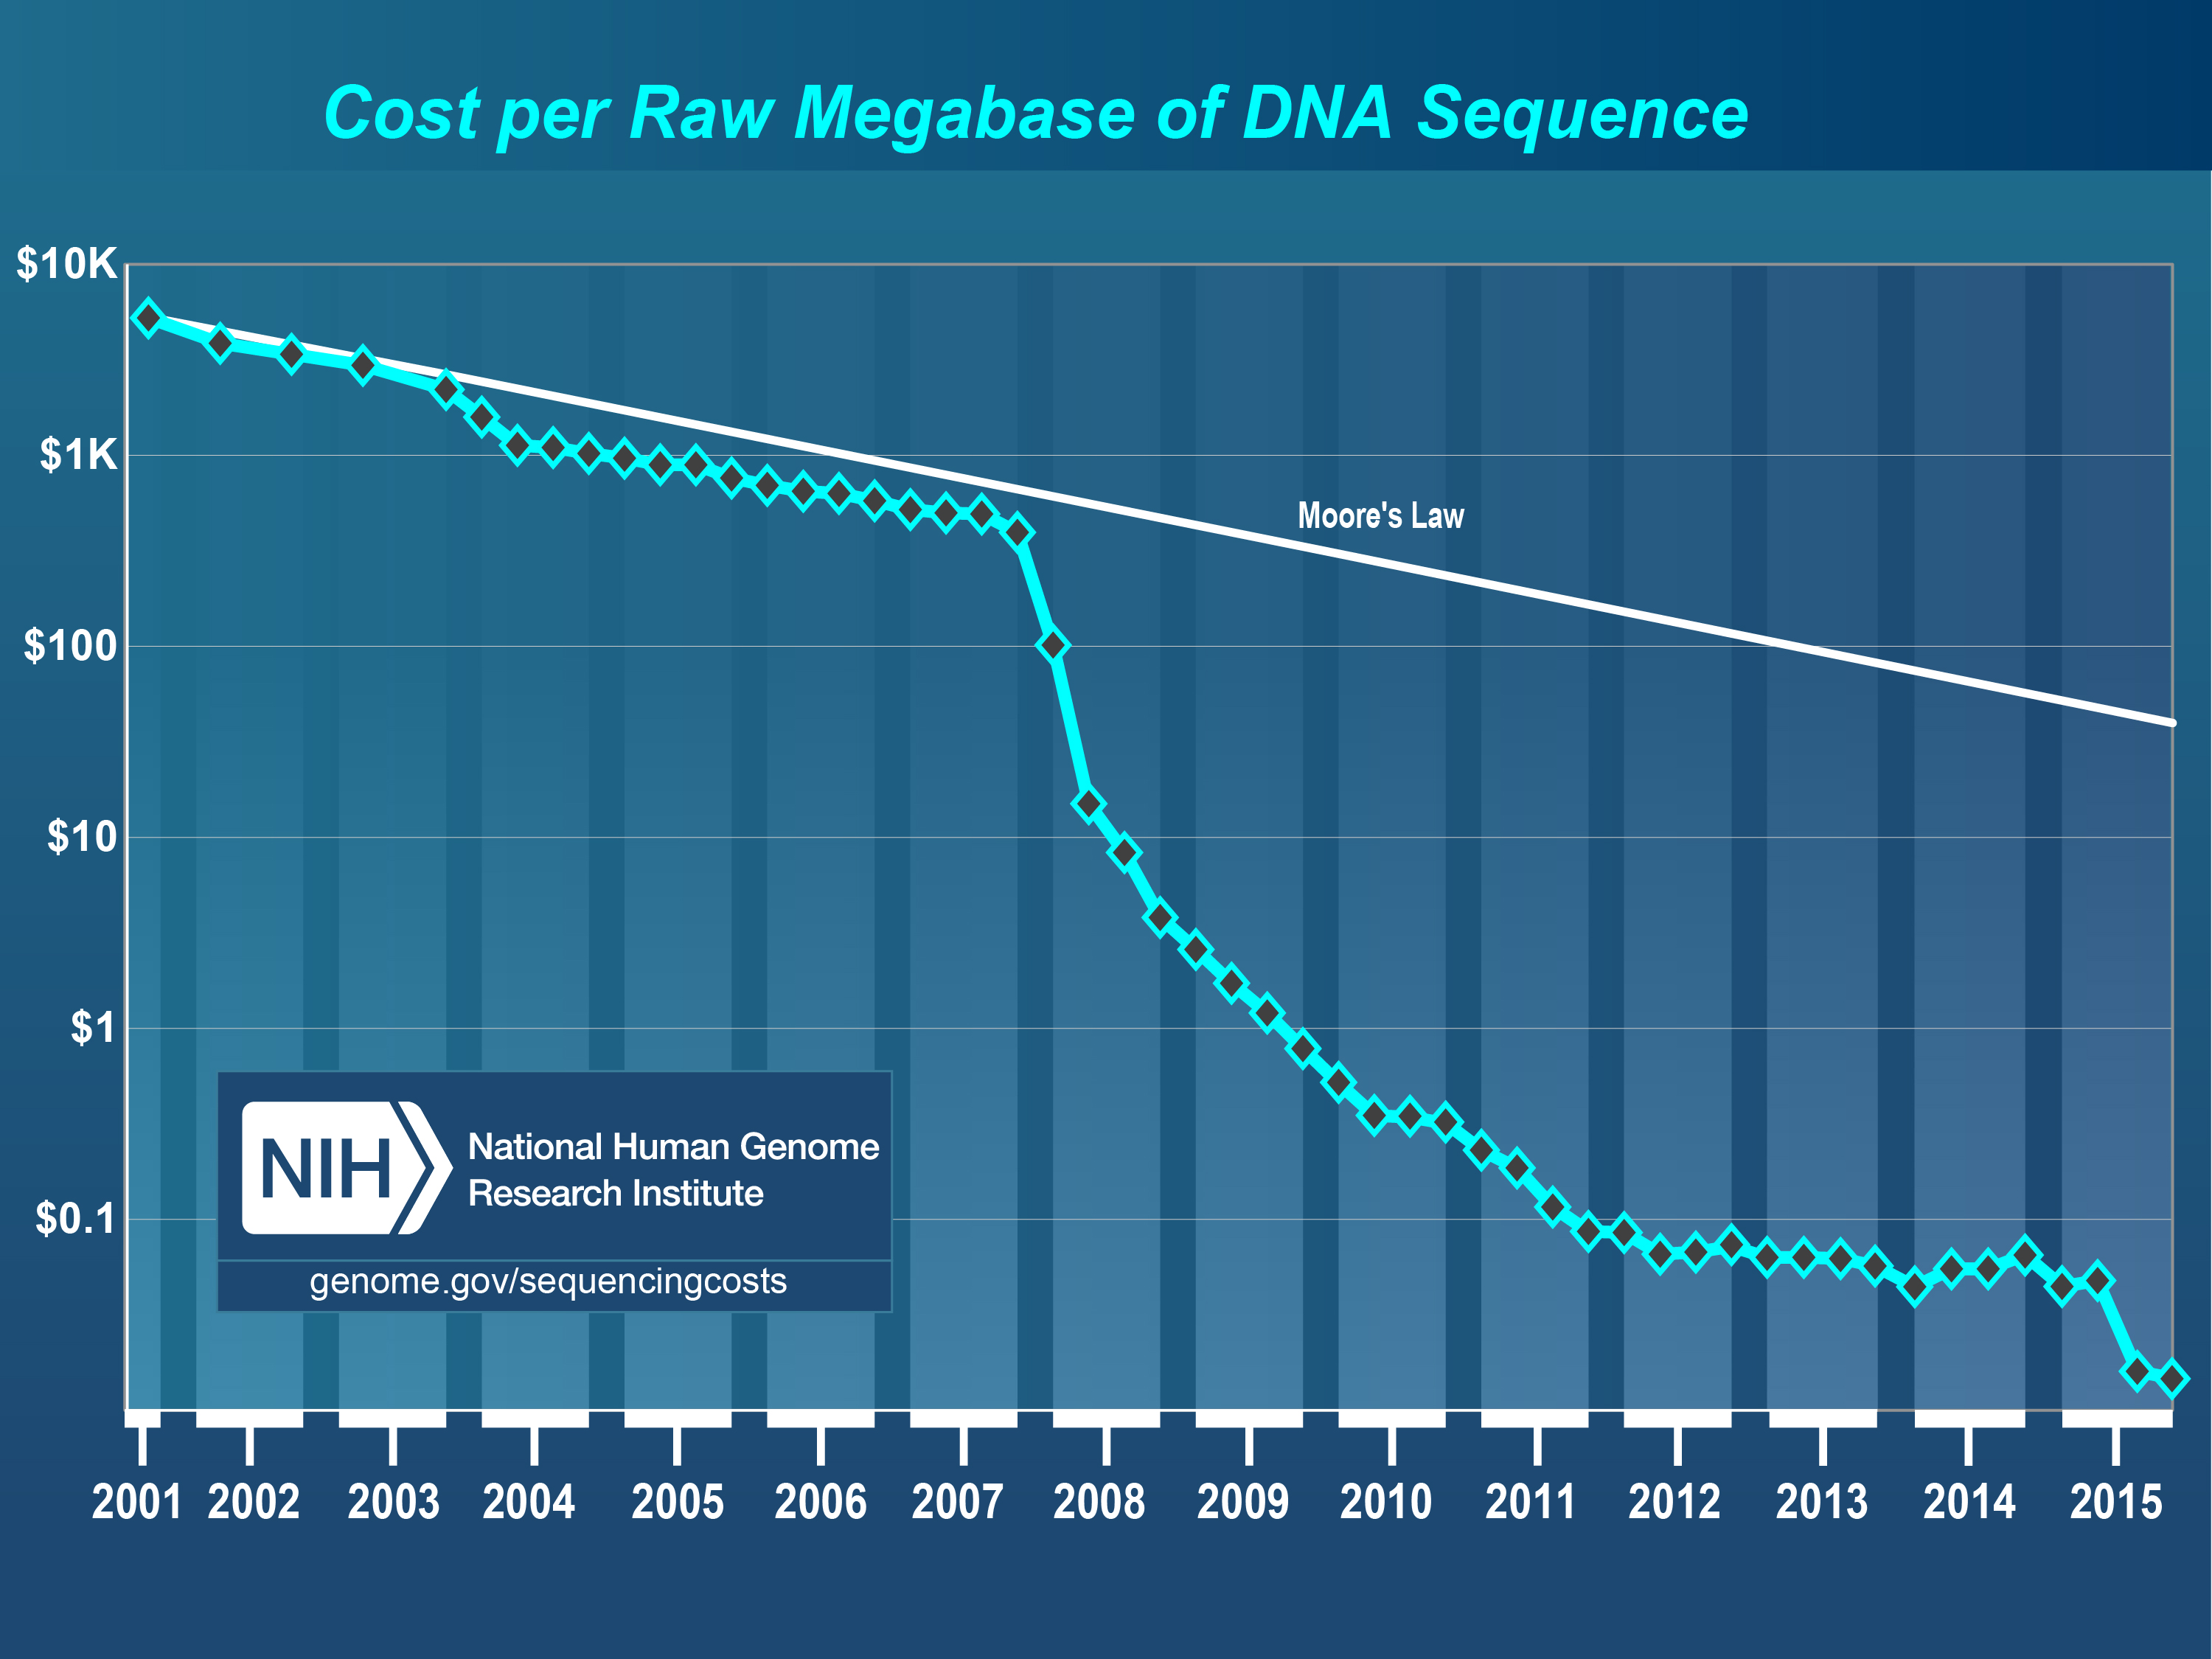
\includegraphics[scale=0.5]{costperMb2015_4.jpg}
% \end{center}
% \caption[Cost per raw megabase of DNA sequence from 2001 to 2015]{Cost per raw megabase of DNA sequence from 2001 to 2015. Straight line - Moore's Law, blue curve - cost in US dollars, Y-axis scale is logarithmic. Graph reproduced from \citep{wetterstrand2016}}
% \end{figure}

% \chapter{}
% \begin{figure}[hb!]
% \begin{center}
% 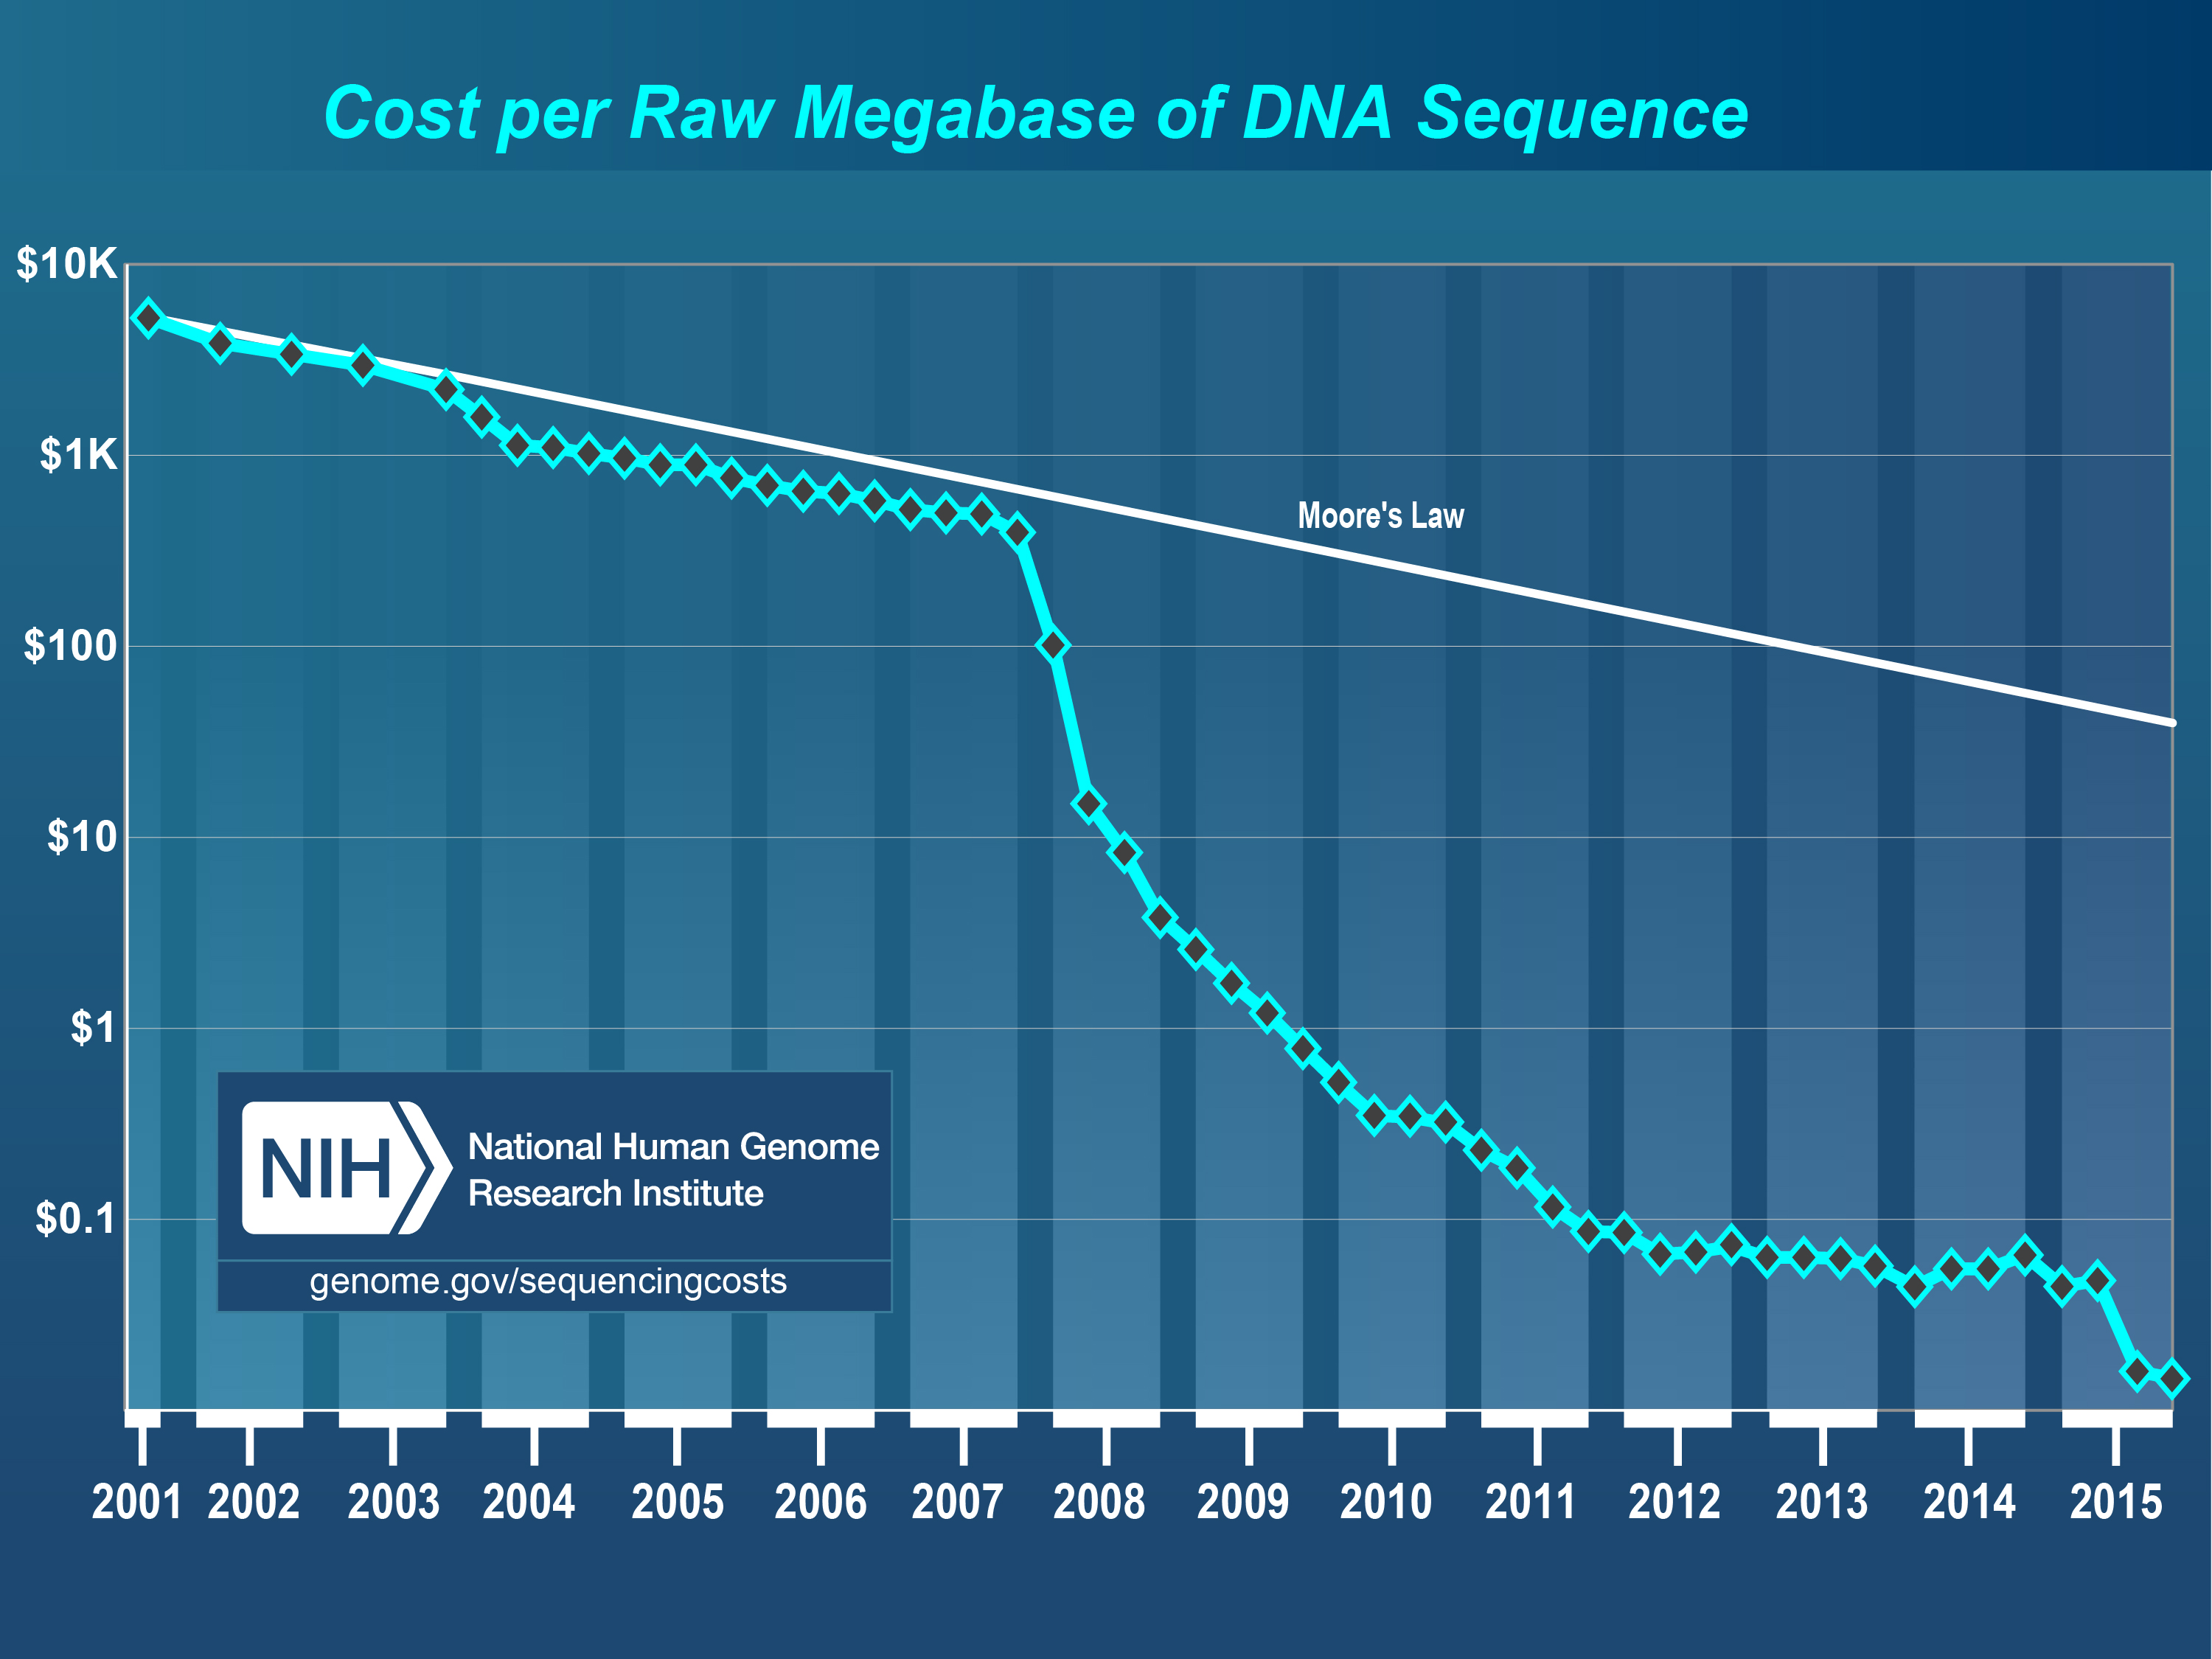
\includegraphics[scale=0.5]{costperMb2015_4.jpg}
% \end{center}
% \caption[Cost per raw megabase of DNA sequence from 2001 to 2015]{Cost per raw megabase of DNA sequence from 2001 to 2015. Straight line - Moore's Law, blue curve - cost in US dollars, Y-axis scale is logarithmic. Graph reproduced from \citep{wetterstrand2016}}
% \end{figure}